%% AL-039 — Geometric Network Pro (LaTeX)
%% Blue profile box, circular photo, geometric background, accent headers
\documentclass[11pt,a4paper]{article}
\usepackage[utf8]{inputenc}
\usepackage[T1]{fontenc}
\usepackage{mathpazo}
\usepackage[margin=0pt]{geometry}
\usepackage{tikz}
\usepackage{xcolor}
\usepackage{fontawesome5}
\usepackage{enumitem}
\usepackage{hyperref}
\usepackage{parskip}
\usepackage{multicol}

% ── Colors ──
\definecolor{blue-pri}{HTML}{3B6BB0}
\definecolor{blue-sec}{HTML}{EBF2FA}
\definecolor{white}{HTML}{FFFFFF}
\definecolor{body}{HTML}{333333}
\definecolor{muted}{HTML}{777777}
\definecolor{border}{HTML}{EEEEEE}

\hypersetup{colorlinks=true,urlcolor=blue-pri,linkcolor=blue-pri,pdfborder={0 0 0}}
\pagestyle{empty}

\begin{document}

\noindent
\begin{tikzpicture}[remember picture, overlay]
  % Geometric background (subtle pattern)
  \foreach \i in {0,2,4,6,8,10,12,14,16,18,20} {
    \foreach \j in {0,2,4,6,8,10,12,14,16,18,20,22,24,26,28} {
      \draw[blue-pri, opacity=0.04] (\i,\j) -- (\i+1,\j+1);
      \draw[blue-pri, opacity=0.04] (\i+1,\j) -- (\i,\j+1);
    }
  }
\end{tikzpicture}

% ═══════════ SIDEBAR ═══════════
\noindent
\begin{minipage}[t]{0.32\textwidth}
\color{body}
\vspace{40mm}
\centering

% Name Box
\begin{tikzpicture}[remember picture, overlay]
  \fill[blue-pri] ([yshift=-230pt, xshift=0pt]current page.north west) rectangle ([yshift=-310pt, xshift=0.32\paperwidth]current page.north west);
\end{tikzpicture}

\vspace{-15mm}
% Photo Placeholder
\begin{tikzpicture}
  \begin{scope}
    \clip (0,0) circle (2.2cm);
    \node at (0,0) {\fontsize{40}{45}\selectfont\color{blue-pri!20}\bfseries ((( (personal.full_name | default('PR', true))[0] )))((( (personal.full_name | default('PR', true)).split(' ')[1][0] if (personal.full_name | default('PR', true)).split(' ')|length > 1 else '' )))};
  \end{scope}
  \draw[white, line width=1.5mm] (0,0) circle (2.2cm);
  \draw[blue-pri!10, line width=0.1mm] (0,0) circle (2.2cm);
\end{tikzpicture}

\vspace{5mm}
{\fontsize{18}{22}\selectfont\color{white}\bfseries ((( personal.full_name | default('Priya Rao', true) )))}\\[25pt]

\raggedright
\hspace{10mm}
\begin{minipage}[t]{0.85\textwidth}
\vspace{10pt}

% ── Contact ──
{\fontsize{11}{13}\selectfont\color{blue-pri}\bfseries \faInfoCircle\space Contact}\\[-4pt]
{\color{blue-pri}\rule{\linewidth}{1.5pt}}\\[10pt]
((* if personal.phone *))
{\small\color{blue-pri}\faPhone\hspace{8pt}\color{body!90} ((( personal.phone ))) }\\[8pt]
((* endif *))
((* if personal.email *))
{\small\color{blue-pri}\faEnvelope\hspace{8pt}\color{body!90}\href{mailto:((( personal.email )))}{((( personal.email ))) }}\\[8pt]
((* endif *))
((* if personal.location *))
{\small\color{blue-pri}\faMapMarker*\hspace{8pt}\color{body!90} ((( personal.location ))) }\\[8pt]
((* endif *))
((* if personal.portfolio *))
{\small\color{blue-pri}\faGlobe\hspace{8pt}\color{body!90}\href{((* if 'http' not in personal.portfolio *))https://((* endif *))((( personal.portfolio )))}{((( personal.portfolio | replace('https://', '') | replace('http://', '') ))) }}\\[8pt]
((* endif *))

\vspace{15pt}

% ── Skills ──
((* if skills and skills|length > 0 *))
{\fontsize{11}{13}\selectfont\color{blue-pri}\bfseries \faChartBar\space Skills}\\[-4pt]
{\color{blue-pri}\rule{\linewidth}{1.5pt}}\\[10pt]
((* for skill in skills *))
{\small\color{blue-pri}$\bullet$\hspace{8pt}\color{body!85}{\fontsize{8.5}{10}\selectfont ((( skill.name )))}\\[4pt]
((* endfor *))
\vspace{15pt}
((* endif *))

% ── Languages ──
((* if languages and languages|length > 0 *))
{\fontsize{11}{13}\selectfont\color{blue-pri}\bfseries \faLanguage\space Languages}\\[-4pt]
{\color{blue-pri}\rule{\linewidth}{1.5pt}}\\[10pt]
((* for lang in languages *))
{\small\color{blue-pri}$\bullet$\hspace{8pt}\color{body!85}{\fontsize{8.5}{10}\selectfont ((( lang.name or lang )))}\\[4pt]
((* endfor *))
((* endif *))

\end{minipage}
\end{minipage}%
\hfill
% ═══════════ MAIN COLUMN ═══════════
\begin{minipage}[t]{0.65\textwidth}
\color{body}
\vspace{15mm}
\hspace{5mm}
\begin{minipage}[t]{0.92\textwidth}

% Professional Summary Box
\begin{tikzpicture}
  \node[fill=blue-pri, text=white, font=\fontsize{11}{13}\bfseries, inner sep=10pt, minimum width=0.92\linewidth, anchor=north west] (header) at (0,0) {\faUser\space Professional Summary};
  \node[draw=blue-pri, inner sep=10pt, minimum width=0.92\linewidth, anchor=north west, align=justify] (content) at (0,-0.8) {{\fontsize{9.5}{14}\selectfont ((( personal.summary | default('Summary goes here...', true) )))}};
\end{tikzpicture}

\vspace{25pt}

% ── Education ──
((* if education and education|length > 0 *))
{\fontsize{12}{14}\selectfont\bfseries\color{blue-pri}\faGraduationCap\space Education} \hfill {\color{border}\rule{0.6\linewidth}{2pt}}\\[10pt]
((* for edu in education *))
\begin{minipage}{\linewidth}
{\fontsize{10}{12}\selectfont\bfseries ((( edu.institution )))} \hfill {\scriptsize\color{white}\setbox0=\hbox{\textbf{((( edu.start_date ))) --- ((( edu.end_date | default('Present', true) )))}} 
\begin{tikzpicture}[baseline=(char.base)]\node[fill=blue-pri, rounded corners=2pt, inner sep=3pt] (char) {\copy0};\end{tikzpicture}}\\[2pt]
{\fontsize{9.5}{11}\selectfont\color{blue-pri}\textit{((( edu.degree )))((* if edu.field_of_study *)) \textbar\ ((( edu.field_of_study )))((* endif *))}} \hfill {\scriptsize\color{muted}\textit{((( edu.location )))}}
\end{minipage}
\vspace{12pt}
((* endfor *))
\vspace{10pt}
((* endif *))

% ── Experience ──
((* if experience and experience|length > 0 *))
{\fontsize{12}{14}\selectfont\bfseries\color{blue-pri}\faBriefcase\space Experience} \hfill {\color{border}\rule{0.6\linewidth}{2pt}}\\[10pt]
((* for exp in experience *))
\begin{minipage}{\linewidth}
{\fontsize{10}{12}\selectfont\bfseries ((( exp.company )))} \hfill {\scriptsize\color{white}\setbox0=\hbox{\textbf{((( exp.start_date ))) --- ((( exp.end_date | default('Present', true) )))}} 
\begin{tikzpicture}[baseline=(char.base)]\node[fill=blue-pri, rounded corners=2pt, inner sep=3pt] (char) {\copy0};\end{tikzpicture}}\\[2pt]
{\fontsize{9.5}{11}\selectfont\color{blue-pri}\textit{((( exp.title )))}} \hfill {\scriptsize\color{muted}\textit{((( exp.location )))}}
((* if exp.description *))\\[4pt] {\fontsize{9}{12}\selectfont ((( exp.description )))}((* endif *))
((* if exp.highlights and exp.highlights|length > 0 *))
\begin{itemize}[leftmargin=12pt, itemsep=2pt, parsep=0pt, topsep=4pt]
((* for hl in exp.highlights *))((* if hl *))\item {\fontsize{8.5}{11.5}\selectfont ((( hl )))}(* endif *)
((* endfor *))
\end{itemize}
((* endif *))
\end{minipage}
\vspace{15pt}
((* endfor *))
\vspace{10pt}
((* endif *))

% ── Awards ──
((* if awards and awards|length > 0 *))
{\fontsize{12}{14}\selectfont\bfseries\color{blue-pri}\faTrophy\space Awards} \hfill {\color{border}\rule{0.7\linewidth}{2pt}}\\[10pt]
\begin{itemize}[leftmargin=12pt, itemsep=2pt, parsep=0pt, topsep=0pt]
((* for award in awards *))
\item {\fontsize{9}{11}\selectfont ((( award.name or award )))}
((* endfor *))
\end{itemize}
((* endif *))

\end{minipage}
\end{minipage}

\end{document}
